\documentclass[tikz,border=10mm]{standalone}
\usetikzlibrary{calc}

\def\xw{5}
\def\yw{4}
\def\rad{5.0mm}

\def\paperxw{2}
\def\paperyw{2}

\begin{document}
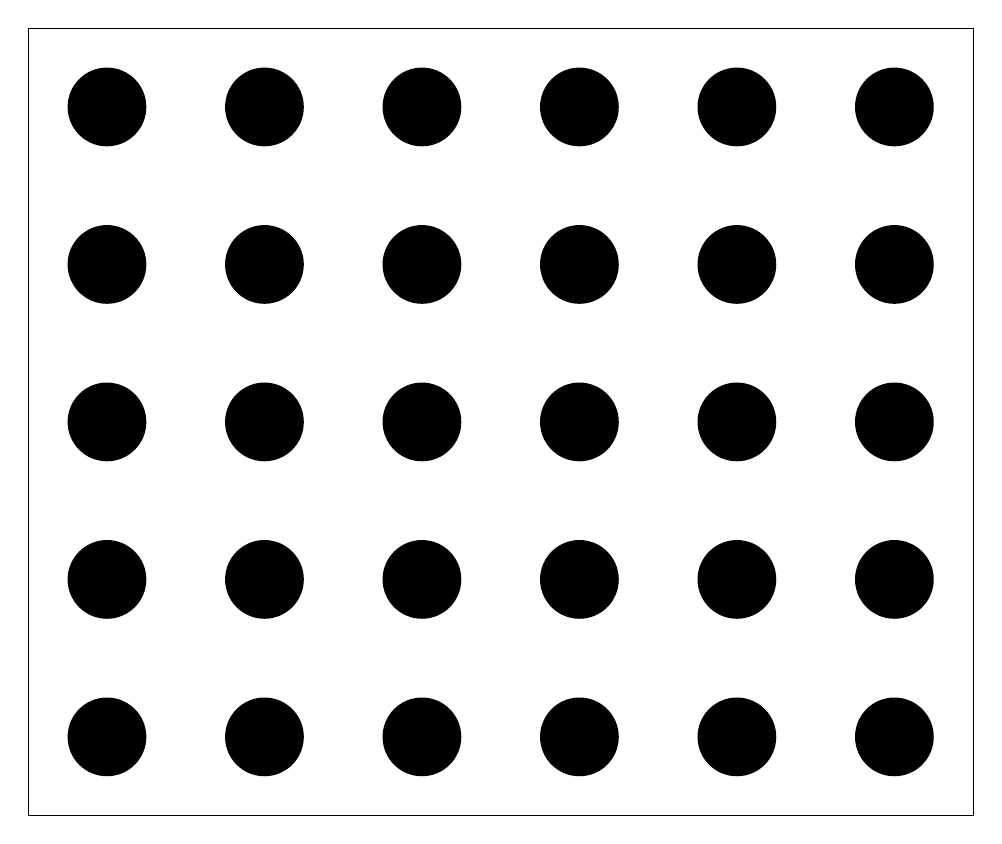
\begin{tikzpicture}[scale=1]






\draw ( 0mm ,0mm) rectangle (\xw*20.0 mm+20.0mm,\yw*20.0 mm +20.0  mm);

\foreach \b in {0,...,\xw}{
   \foreach \c in {0,...,\yw}{
      \fill[black] (\b*20.0mm+10mm,\c*20mm+10mm) circle [radius=\rad] ;
    
    }

}


\end{tikzpicture}
\end{document}
\geometry{letterpaper}
